\chapter{Literature Review: Image Recognition Models and Interpretability}
\label{ch:rel}
\chaptertoc{}
\section{Introduction}
Image recognition models capabilities have improved with constant development, 
closely aligned with the increase in computing power. This evolution has lead to steady 
advancements in both performance and complexity. On its early approaches, image recognition models 
relied on handcrafted feature extraction methods  in conjuction with traditional machine learning 
algorithms. However, this reliance on these features ultimately limits these methodologies' 
capabilities to capture intricate visual patterns.
On particular, one approach that had a strong initial impact and high performance was \gls{hog} 
\autocite{dalal2005histograms}. In this methodology, gradient information was used to train a 
\gls{svm} to perform pedestrian recognition. While achieving high performance in the dataset it was 
designed, \gls{hog} ultimatately failed in data collections where complexity was higher 
\autocite{5975165}.\\
Furthermore, with the resurgence of convolutional neural networks and the ensuing advent of 
deep learning, a paradigm shift in this field occurred. This transition led to the elimination of 
the need for handcrafted feature extraction; instead, deep learning allowed \glspl{cnn} to act 
as both feature extractor and classifiers on themselves. Moreover, based on the aggregation of 
convolutions as their fundamental units, a \gls{cnn} is able to learn hierarchichal 
representations of data, extracting intricate features directly. 
Consequently, this shift resulted in improvements in accuracy and performance in various image 
recognition tasks. \\

\noindent In \autoref{rel:sec_imrecon} we explore some of the most important approaches based 
on machine learning designed towards image recognition. In particular, in \autoref{rel:sub_cnn}, we 
introduce the basis of deep learning and \glspl{cnn}. Moving on, in \autoref{rel:sub_att} we make 
mention of the Transformer architecture, its building block and how it has reshaped the landscape 
of image recognition. Finally in \autoref{rel:sub_hybrid} we display approaches that make use of 
combinations of the last two forementioned approaches.\\


\noindent With the adoption of deep image recognition into society; understanding the 
innerworkings of these models has become a top priority. We shine light into some fields where 
this is the case:
\begin{itemize}
    \item \textbf{Facial Recognition} Facial recognition is a fine grained classification task, 
    that can be mostly associated with identification and re-identification of individuals. 
    In this aspect, understanding model predictions is associated with accountability, ethical 
    considerations and safety.
    (\cite{selinger2020inconsentability}, \cite{andrejevic2020facial}).
    \item \textbf{Automated Medical Diagnosis} In medical imaging, the education 
    required to read and provide analysis, often requires experience based 
    on personal expertise \autocite{nakashima2013visual}. Examples of automated diagnosis encompas 
    melanoma detection, bone age assessment and most recently, COVID-19 diagnosis 
    (\cite{yu2016automated}, \cite{BoNet2019hand}, \cite{huang2021artificial}). The medical domain 
    is of special care as human lives are directly at stake, therefore understanding predictions is 
    highly desired.
    \item \textbf{Self-driving Vehicles} Over the past decade, advancements in this field have lead to 
    discussions regarding the impact of the adoption of these kind of vehicles within smart cities  
    (\cite{duarte2018impact}, \cite{millard2018pedestrians}). Nevertheless their 
    navigation is not completely perfect and it is also possible to attack it, leading to possible 
    traffic accidents \autocite{dixit2016autonomous}; in this case, accountability is then again 
    taken into consideration.
\end{itemize}

We observe that interpretability needs in these fields and real world applications follows 
Lipton's discussion on the \textit{Desiderata of Interpretability Research} 
\autocite{mythos_interp}. In this aspect, we expect that the explanations that any given 
approach help us \emph{trust} any model. Conversely, we expect a model to be explained in a 
\emph{causal} manner according to its explanations. On another hand, 
we expect these remarks be \emph{informative} and shine light on similar examples that the 
model processes. Finally, we expect interpretable explanations to guarantee that the outputs 
of a model are \emph{fair} and \emph{ethical}.

With these properties in mind leading the \emph{desiredata of interpretability study}, we further 
investigate in this work some of the most important works on interpretability. In 
\autoref{rel:sec_int} we explore preliminary ideas of this field. Delving deeper, in 
\autoref{rel:sub_transp} we discuss efforts aimed at transparency of machine learning approaches. 
In contrast, \autoref{rel:sub_post} we explore and study 
some of the most relevant studies on post-hoc interpretability. Conversely, in 
\autoref{rel:sub_evl}, we outline the evaluation metrics used for evaluation the aforementioned 
works. To understand how these proposals are evaluated in their claims of interpretability, we 
introduce and explain evaluation methodologies in \autoref{rel:sub_evl}.
%\addcontentsline{toc}{chapter}{Literature Review}
%--------------------------------------------------------------------------------------------------
\section{Image Recognition Models}
\label{rel:sec_imrecon}
Image recognition is a substask of computer science that aims at replicating human vision capabilities 
with a machine. Arguably, it is with the improvement and interaction of the three fundamental tasks 
of computer vision (Recognition, Reconstruction and Reorganization) \autocite{malik2016three} that we 
find this field moves forward. Interestingly, improvements in one these fundamental Rs can be 
used to drive forth its peers; moreover, (words).




%1960s, first thesis, image processing, pattern recognition
%1970s foundational work on image recognition
%1980 vision applied to maths, geometry, control theory, optimization
%1990s geometric analysis coplete, graphics,statistical learning
%200s advances in visual recognition, practical applications

Ultimately, it was with inspiration on studies on neuroscience \autocite{hubel1959receptive} that the 
development of \glspl{nn} started. In particular, the Neocognitron \autocite{fukushima1975cognitron} 
proposes the first \gls{nn} where kernel operations, feature aggregation in a hierarchical 
manner and non-linearities stand out as these contributions can be seen as the main components of a 
most recent image recogniton models.

Still, the Neocognitron's hierarchical properties and aggregation didn't really achieve 
a great deal of momentum on early days; around this time, other image recognition models were being 
used yielding better results, examples of this can be seen with the amount of traditional machine 
learning based methods that dominated this task around that time. Still getting close to the dawn 
of the 1990s, Yann LeCunn proposed LeNet to perform digit recognition \autocite{lecun1998gradient}.\\

\subsection{Convolutional Neural Networks}
\label{rel:sub_cnn}
Starting with LeNet, the convolution took prominence as the fundamental building block 
of most current image recognition models. On itself, a convolutional layer operates by the 
interaction of a kernel with a set of features at any given layer. This interaction depends in 
direct correlation with the kernel size, mediated by its width and height. Furthermore, 
these kernels are meant to project features into different spaces; with this in mind we point out 
that convolutions are mostly a local operation. 
%Figure \ref{fig:conv_local} illustrates these 
%properties of the convolution operation.
%\begin{figure}[h]
    \centering
    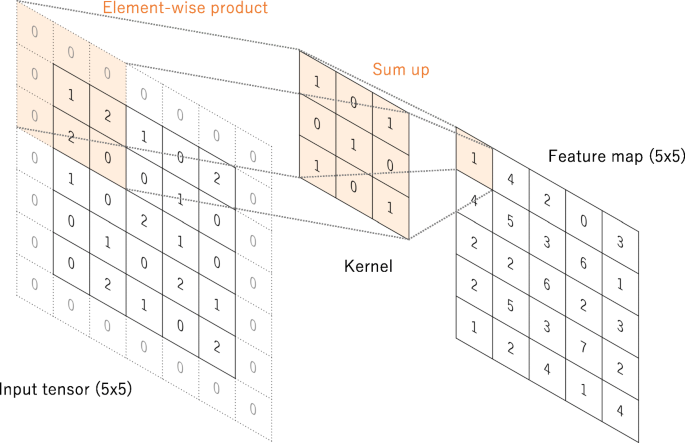
\includegraphics[width=\textwidth]{fig/rel/images/conv_not_proper.png}
    \caption{Illustration of the convolution operation. Properties, parameters and behaviour.}
    \label{fig:conv_local}
\end{figure}

\noindent On top of convolutions, LeNet led to the introduction of more components of \glspl{cnn}: 
pooling operations and non-linearities. Pooling operations are used to reduce the spatial 
resolutions of feature maps, which in turn aids convolutions in capturing features from longer 
range dependencies within the image. Moreover, via pooling it is possible to capture the most 
relevant features within a neighborhood.

On another hand non-linearities such as Sigmoid and ReLU, are designed to capture complex 
relationships within data and stop the model collapsing into a linear operation. Moreover, these 
operations also contribute with stability: they maintain values within feature maps and the gradient 
in ranges in which the network can operate with. %cite this?
Still, the key contribution leading to the success of LeNet was not only the usage of 
convolutions, pooling and nonlinearities; but its training process, that guided by gradient to 
optimize ultimately enabled \glspl{cnn} to outperform traditional computer vision methods for document 
recognition. \\

\noindent With the advent of the 2010s and the organization of the \gls{ilsvrc} \autocite{ILSVRC15} 
a proper environment for further devolpement of models was found. Unlike prior datasets in the 
time, ImageNet was composed of images that presented more complexity than earlier datasets; instead 
of catalogue-like compositions, for instance, elements in this dataset are closer to those found in 
the wild by having multiple classes or instances of a class in one  image. Upon its release, 
several traditional approaches were trained and evaluated in this collection, achieving a low 
performance. Nevertheless, \glspl{cnn} returned to the front of image recognition with the 
introduction of AlexNet \autocite{krizhevsky2012imagenet}. Inspired by LeNet, Krizhevsky designed a 
\gls{cnn} that added a few more convolutions but most importantly, allowed for a more eficient 
convolution by effective communication with the \gls{gpu}.



 LeNet \cite{lecun1998gradient}, AlexNet \cite{krizhevsky2012imagenet}, VGG \cite{simonyan2015deep}, ResNet \cite{he2016deep}, 
Inception (\cite{szegedy2015going}, \cite{szegedy2016rethinking}), NasNet (\cite{zoph2018learning})
EfficientNet(\cite{tan2019efficientnet}) 
ResNet Strikes back (\cite{wightman2021resnet}) \autocite{liu2022convnet}
%\addcontentsline{toc}{subsection}{Convolutional Neural Networks}

\subsection{Attention-Based Architectures}
\label{rel:sub_att}
%\addcontentsline{toc}{subsection}{Attention-Based Architectures}
Attention is a powerful mechanism that has been introduced into convolutional networks in several 
ocasions (\cite{bello2019attention}, \cite{ramachandran2019stand}, \cite{shen2020global}). 
With the success of vision transformers (ViT) (\cite{dosovitskiy2020image}), fully attention-based 
architectures are now competitive with convolutional networks. To benefit from both self-attention 
and convolutional layers, some hybrid architectures employ convolutional layers before the vision transformer 
. Others, such as Swin (\cite{liu2021swin}) and PiT 
(\cite{heo2021rethinking}), introduces a pyramid structure to share local spatial information 
while reducing the spatial resolution, as in convolutional networks. 

SCOUTER (\cite{li2021scouter}) uses slot attention (\cite{locatello2020object}) to build a class 
specific pooling mechanism, which does not scale well to more than 20 classes. 

\subsection{Hybrid Architectures}
\label{rel:sub_hybrid}
(\cite{graham2021levit}, \cite{xiao2021early})
Conformer (\cite{peng2021conformer}) proposes a dual network structure to retrain and fuse local 
convolutional features with global representations. Our method merely provides a simple 
attention-based pooling mechanism inspired by transformers that can work with any architecture, 
even pretrained and frozen. PatchConvNet (\cite{touvron2021augmenting}) replaces global average pooling by an 
attention-based pooling layer.

\newpage
%--------------------------------------------------------------------------------------------------
\section{Interpretability}
\label{rel:sec_int}
As deep learning based models for Computer Vision have continued to improve in their recognition 
properties, their structure and functioning have become more opaque; in turn making these 
technologies seen as black boxes. A black-box model is defined as a model for which its 
interpretation is not straightforward for humans \autocite{petch2022opening}. In recent years 
with the assimilation of deep learning into everyday tasks, and the implicit effect these models 
are having on human lives; the novel research field of \emph{Interpretability} has been brought 
forth to open up this black-box behaviour. Scholars have approached intepretability alongside 
different directions. Starting with the work of \cite{li2018deep}, interpretability is suggested 
to present two categories, \emph{Transparency} and \emph{Post-hoc Interpretability}.
For the former, Lipton argues that it follows modifications of the model or the training process, 
in order to explain the inner-workings of the model. Conversely, for the latter Lipton builds upon 
the black-box behaviour of the model, providing explanations istead based on inputs and outputs; 
without adding any further modifications for the model or altering its training process.\\

Complementary to Lipton's proposal, \cite{guidotti2018survey} points that interpretability is 
contained along different dimensions. On one hand, a model can be understood on its entirety 
following a \emph{Global} interpretation; whereas in situations where only the reasons leading to a 
specific prediction, a \emph{Local} interpretation is found. Guidotti also considers time,
more specifically \emph{Time Limitation} as its availability is strictly correlated to the scenario 
where the model is used. Finally, the \emph{Nature of User Expertise} covers the last dimension of 
interpretability; where knowing the experience of an user in a given task is considered to be a 
key aspect describing the interpretability of a model.\\

In recent years, \cite{zhang2021survey} suggested that three different dimensions encompass this 
study. The first dimension answers to the nature of an approach; where it can be either 
\emph{Passive} or \emph{Active}. The first direction in this dimension correlates to Lipton's 
\emph{Post-hoc interpretabity}, the latter follows the aforementioned \emph{Transparency} property.
Zhang's second dimension is addressed towards the type of explanations, where the order of 
explanatory power follows a hiearchy starting on its base level with examples, into attributions, 
leading into hidden semantics and finishing in rules. The last dimension that Zhang covers 
explanations in the input space, where a \emph{Local} explanation describes the network's 
prediction following individual samples; while on another hand, a \emph{Global} explanation 
describes the network as a whole. This last dimension is similar to the first point described by 
\cite{guidotti2018survey}. Most importantly, Zhang's dimensions are not used separatedly to 
categorize an approach, instead according to the methodology propierties and the nature of the 
explanation provided. This is further seen in the 3D space found in \autoref{fig:rel_zhangs}

\begin{figure}[H]
    \centering
    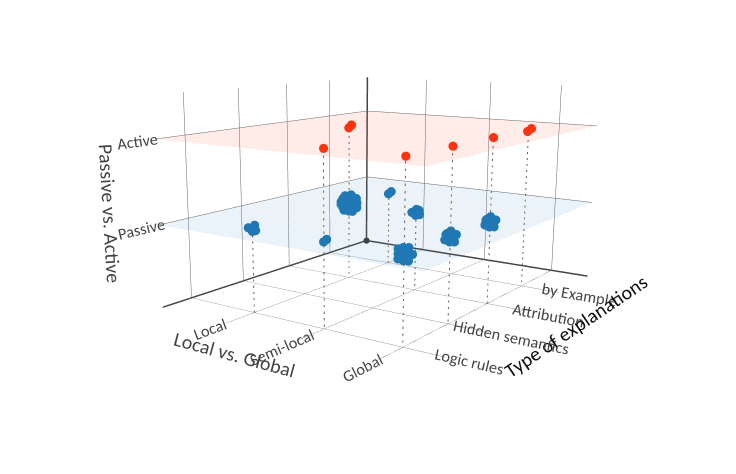
\includegraphics[width=0.8\textwidth]{fig/rel/images/ZhangsInterpspace.png}
    \caption{Interpretabiltiy studies grouped by nature. Source from \url{https://yzhang-gh.github.io/tmp-data/index.html}}
    \label{fig:rel_zhangs}
\end{figure}
 
In this thesis we study interpretability according to Lipton's properties; nevertheless, as shown 
in the following subsections, we aknowledge their strengths and weaknesses, while noting some of 
the most prominent works in each dimension. In \autoref{rel:sub_transp} we discuss 
\emph{transparency}, its properties according to Lipton and its difficulties describing deep models, 
alongside a survey following Zhang's active dimension. Conversely, in \autoref{rel:sub_post}, we 
study \emph{post-hoc interpretability} in a similar fashion to transparency.

\subsection{Transparency}
\label{rel:sub_transp}
Following Lipton's work, we further define the transparency property of models as the opposite of 
opacity or black-box behaviour. Still, similar to the aforementioned works, transparency is 
considered at the model level (\emph{simulatability}), individual components 
(\emph{decomposability}) and the training algorithm (\emph{algorithmic transparency}). Delving into 
detail, \emph{Simulatability} on a strict definition answers to the capability of a model to be 
fully contemplated by an individual on its entirety at once. Currently, with the increase of model 
complexity this understanding level is then redefined as the capcity of a model to be readily 
presented to an user with visual or textual artifacts. This in turn can be demonstrated by 
\emph{post-hoc interpretations}.\\

Regarding \emph{decomposability}, Lipton suggests that an interpretable model has to present 
an intuitive explanation, regardless of it being an input, parameter or calculation. In this 
dimension it is then stated that a computation follows an association between features, in 
accordance to \emph{intelligibility} as proposed in \autocite{lou2012intelligible}. Still, Lipton 
also points that this notion should not be accepted blindly as some parts of the computation steps 
can be fragile processing and calculation; for instance, image normalization can lead to prediction 
mismatch during inference.\\

Finally, Lipton argues that \emph{algorithmic transparency} applies on the level of the learning 
algorithm itself. In short, this applies to the er ror surface and assumption of the existence of 
an optimal and/or unique solution to the problem. Nevertheless this dimension is not met for deep 
learning models as the training process is not completely understood.\\

\noindent While Lipton's transparency properties appear to be applicable and theoretically sound, 
transparency is not fully studied alongside them. As previously observed, designing an approach or 
model covering these properties is a complicated task for deep models. However, with a bfief 
modification of their definition, transparent properties can be further applied to deep image 
recognition. \emph{Simulatability}, as mentioned earlier,  can be supported with \emph{post-hoc 
interpretability} explanations. Conversely, deep learning models can be further 
\emph{decomposed} into functional units; for instance, the ResNet architecture consists of
residual blocks, where the structure of each block and its design has been studied thoroughfully. 
Finally, concerning \emph{algorithmic transparency}, although deep learing models present high 
dimension error surfaces and a high amount of local minima; still, ensuring a deterministic 
behaviour leads to replicability, in turn demonstrating part of the training process.\\

\noindent Following the interpretable dimensions described by \autocite{zhang2021survey}, 
transparency is suggested as an active change of the network's architecture or the training process 
in order to provide explanations. Furthermore, according to the type of explanations provided by an 
interpretable approach, transparency methods can be explained according to logic rules, hidden 
semantics, attributions and explanations by example.\\

\noindent \emph{Rule-based methods.} In this group, rules are used to provide an explanation. 
To do this, Wu et al. proposed training a decision tree on top of a deep learning model, acting as 
a regularization term and an aproximation of said deep model (\cite{wu2018beyond}, 
\cite{wu2020regional}). This process involves two steps. First a binary tree is trained, mapping 
inputs to the model's prediction. The second part of this approach calculates the average path 
length between root to leaf nodes on the decision tree, covering all data points. Ultimately, Zhang 
argues that this regularization improves interpretability by forcing a model to be described by a 
decision tree.\\

\noindent \emph{Hidden semantics-based methods.} This family of methods focuses on the filters 
and properties found alongside in different depths of the model. These approaches are based in 
observations of filter response to inputs at different depths, and the semantic information 
contained by them(\cite{bau2017network}, \cite{zhou2018interpreting}). 
One particular approach studying this is that of \autocite{zhang2018interpretable}, introducing a 
loss term that encourages deep filters to represent a single concept. More recently, as an answer to 
semantics only being extracted from deep layers, and the information flow not being taken into 
consideration to provide an explanation; the work of B\"ohle et al. (\cite{bohle2022b}, 
\cite{bohle2024b}) introduced the idea of \emph{B-Cos networks} and alignment overall with the 
\emph{Dynamic Alignment Unit}. In these works, alignment between weight-input alignment is 
emphasized by the inclusion of the B-cos transform and dynamic alignment unit. Moreover, the 
interpretations these methods provide insight over the entirety of the network and they are 
possibly integrated into existing architectures.\\

\noindent \emph{Prototype-based methods.} On this topic, Li et al. designs an architecture that 
incorporates an autoencoder and a standard classification network \autocite{li2018deep}. 
In detail, the autoencoder reduces dimensionality of inputs, producing high quality features for 
classification. The encoded features are then used to produce a probability distribution over the 
dataset classes. Interestingly, during the forward pass on the prototype network, these encoded 
features are transformed into prototype vectors; ultimately used to train the classifier. Therefore, 
the classification algorithm is distance-based on the low dimensional learned feature space. 
Another approach showcasing prototype learning is that contained within \emph{This Looks Like That} 
\autocite{chen2019looks}. In this approach, Chen proposes a prototype layer that learns prototypes 
on top of existing architectures, aligning learn a set of prototypes to specific categories. 
or parts as an intermediate representation in the network, which can be aligned with categories.
One difficulty these prototype parts face, is their heavy computation and difficulty to 
train. As a response of this, ProtoPool \autocite{rymarczyk2022interpretable} is recently proposed, 
allowing for prototype reutilization and differentiable assignment of prototypes to classes; 
speeding up the training process\\

\noindent \emph{Attribution-based methods.} Similar to the regularization induced by the inclusion 
of decision trees, local attributes are improved during training through regularization 
(\cite{ismail2021improving}, \cite{Zhou_2022_BMVC}, \cite{ross2017right}, 
\cite{ghaeini2019saliency}, \cite{lee2021lfi}). These methods are often used in conjunction with 
\emph{post-hoc interpretability} approaches, where an observation made on the explanation proposal 
is further taken into consideration to be modified during training. For instance, on LFI-CAM 
\autocite{lee2021lfi},  an attention branch is included to learn attention feature importance 
during training; allowing for a straightforward saliency map computation while improving 
recognition properties. Similarly, saliency-guided training (\cite{ismail2021improving}) 
minimizes the KL divergence between the output of original and masked images. \\


\subsection{Post-Hoc Interpretability}
\label{rel:sub_post}
According to Lipton, post-hoc interpretability provides information directly from learned models. 
Complementary to this, Zhang points out that \emph{passive} interpretability methods extract 
logical rules or understandable patterns from models. As noted in \autoref{fig:rel_zhangs} a 
discrepancy in the ratio of \emph{active-passive} methods exist, where the \emph{passive} 
dimension presents more studies. Furthermore, according to the nature of 
explanation Lipton groups methods into \emph{textual explanations}, \emph{visualizations}, 
\emph{explanations by example} and \emph{local explanations}. On one hand Lipton argues that 
humans justify decisions verbally, suggesting it is possible to train a model to generate 
explanations describing the predictions of another model. For instance, \gls{nlp}-based approaches 
for image captioning can be utilized to provide textual explanations \autocite{mcauley2013hidden}. 
Nevertheless, in recent years image-captioning approaches have become increasingly complex,
introducing a degree of uncertainty into the explanations provided, as these recent systems 
are now transformer-based and their interpretability is not comprehensively studied yet. Lipton 
closes this discussion addressing that this kind of interpretations are open to scrutiny 
\autocite{chang2009reading}.\\

To provide interpretations on a visual manner according to Lipton, we observe \emph{explanations 
from visualization}, \emph{explanations by example} and \emph{local explanations}. The goal of 
explanations from visualization is to determine qualitatively what the model has learned. One 
instance of this is found on the work by \cite{mahendran2015understanding}, where an image is 
forwarded through a discriminative \gls{cnn} generating a representation. The authors then 
demonstrate that the original image can be recovered from deep-level representations by performing 
gradient descent on randomly initialized pixels.\\

Complementary to \emph{explanations by visualization}, Lipton proposes \emph{explanations by 
example}. These explanations are derived from explaining decisions for a model using examples 
deemed the most similar. In detail, once a model is trained it is possible to extract information 
from learned representations; these in turn can be used to explain a new sample by its proximity 
in this representation space to similar observations. On deep image recognition models, we observe 
the works of (\cite{kim2014bayesian}, \cite{doshi2015graph}), where case-based approaches are 
proposed for interpreting generative models. More recently, the work proposed by 
\cite{rombach2020making}, where an Invertible Neural Network is connected at different stages of a 
model, disentangling deep representations and providing an inverse transformation into accessible 
semantic concepts which can be used to point at similar examples of a given input.\\

Regarding \emph{local explanations}, Lipton aknowledges that describing the entirety of the 
mapping by a \gls{cnn} is a difficult endeavour; and as such, it can be explained on a 
\emph{local} manner. This local behaviour is widely consider across interpretability studies, as 
previously mentioned in \autoref{rel:sec_int} (\cite{guidotti2018survey}, \cite{zhang2021survey}). 
Generally speaking, local explanations are often extracted via the computation of a \emph{saliency 
map} highlighting the most important regions on an image describing a prediction. Studies describing 
local explanations are varied and many of them are build on top of transparency approaches; where 
salient properties can be enhanced via training or optimization. Conversely, local explanations 
are grouped into: gradient-based methods, learning-based methods, masked-based methods and 
class activation based-methods.\\

\noindent \emph{Gradient-based methods.} This family of approaches leverages the property of 
image recognition models, wherein forwarding an example through a model allows for the 
visualization of the response of its weights during backpropagation in correlation to a specific 
prediction. This response is visualized in input space, where strong gradient information is 
expected in regions of the image containing information relevant to the corresponding prediction 
(\cite{baehrens2010explain}, \cite{simonyan2013deep}). However, gradient information often contains 
noise, making it challenging to interpret these modifications in a straightforward fashion 
\cite{adebayo2018local}. Consequently, modifications to backpropagation calculation have 
been proposed, including considering only positive values \autocite{guidedbackprop}, adding noise 
on the input space for denoising \autocite{smilkov2017smoothgrad}, introducing rules and axioms to 
constrain the computation \autocite{sundararajan2017axiomatic} and proposal of concepts like 
relevance \autocite{bach2015pixel} to compute the importance pixel interaction leading to a 
prediction \emph{(LRP)}.\\

\noindent \emph{Learning-based methods.} Approaches in this family of methods exhibit a behaviour 
intersecting  \emph{transparency} based approaches, where an additional network or branch is 
learned atop an existing architecture to produce an explanation map for a given input. However, 
the lack of modifications on the model for interpretation is the key factor differentiating these 
approaches from \emph{active} interpretability methods. Specific examples of learning methods 
comprise modifications inclusion of generative models to fill in information ocluded from  the 
classifier \autocite{chang2018explaining}, masking salient points on the map to manipulatie scores 
on the classifier \autocite{dabkowski2017real}, inclusion of a \emph{masker} side network to 
collect information on different levels of the network and produce a high resolution explanation 
\autocite{phang2020investigating}, addition of a decoder to generate masks and a different 
classifier predicting the masked inputs \autocite{zolna2020classifier}, and finally, a bottleneck 
on top of intermediary layers of the network to learn a saliency map per sample at the specific 
depth of the network \autocite{schulz2020restricting}.\\

\noindent \emph{Occlusion or masking-based methods.} Continuing on with modifications on the input 
space, by purposefully masking certain regions on the image and measuring the subsequent loss in 
predictive power, a saliency map can be produced. In particular, the masking process can provide 
extremal perturbations by measuring the maximal effect upon the activation of neurons leading to 
predictions (\cite{fong2017interpretable}, \cite{fong2019understanding}) masking in feature space 
to provide saliency maps from intermediate stages \autocite{schulz2020restricting}, learning a 
simple masking model around the prediction to provide saliency maps that are locally faithful to the 
classifier \autocite{ribeiro2016should} and iteratively by random masking the input image, probing 
the model and obtaining a saliency map from the linear combination between prediction weights and 
the random mask that was used to generate them. \\

\noindent \emph{\gls{cam}-based methods.} By taking into consideration feature map information 
contained across different layers of a network, it is possible to gain insight into which image 
regions are highlighted at different depths within the model. However, understanding feature maps, 
which are often high-dimensional, present a considerable challenge. On another hand, information 
contained from the classifier layers of the model can be directly associated with classes. For 
example, the product of the weights of the classifier and the last feature map before \gls{gap} 
can generate a saliency map, known as \glsfirst{cam} \autocite{zhou2016learning}. These approaches 
typically utilize feature information from deep layers in conjuction with a set of weights 
correlated with class information to compute explanations (\cite{selvaraju2017grad}, 
\cite{chattopadhay2018grad}, \cite{wang2020score}, \cite{axiombased}, \cite{ablationcam}
\cite{jiang2021layercam})\\

\noindent \emph{Attention-based techniques.} Given the innate properties of attention based 
architectures, most interpretability methods are ill fitted towards explaining the inference 
process of these models. Nevertheless, with the current design of these models it is possible to 
address salient information, although in a class-agnostic manner. In particular, in the computation 
of self attention, this information is highlighted by the product of \emph{query} and \emph{key} 
vectors by focusing on the \Th{[CLS]} token; this in turn is called \emph{Raw Attention}. 
Conversely, since attention is computed at every layer of a transformer, the flow of information 
can be traced across different layers across the network in an approach named \emph{Rollout 
Attention} \autocite{abnar2020quantifying}. Inspired by \emph{rollout attention} and gradient 
methods such as \emph{LRP} \autocite{bach2015pixel} and the indadequacy property of CAM methods on 
transformers, a novel computation of relevance across layers providing high quality attribution 
maps is introduced, allowing at the same time for a quantitative study of the interpretable 
properties of these methodologies \autocite{chefer2021transformer}.\\

In this thesis we take particular interest in proposing and evaluating our interpretability 
methodologies based on \gls{cam}. In particular, we find CAM to be an appealing approach because of 
its ease of use and adaptation to interpret existing models. Moreover, it can be argued that while 
it is possible find and use a plethora of the most popular models towards recognition; providing 
explanations ought to be similarly easy to use, a property that CAM-based models share.
%--------------------------------------------------------------------------------------------------
\paragraph{CAM-based saliency maps}
One property that \glspl{cnn} display is the presence of semantic information found within the 
deepest layers prior to the classifier. In detail, it has been observed that these kind of models 
operate in a similar manner to the visual cortex in the brain; basic textures and their orientation 
is processed in shallow layers, whereas deep layers associate this information into concepts 
\autocite{hubel1959receptive}. This characteristic in turn is the main motivation behind making 
use of CAM methods: by addressing interpretations on the layers prior to the classifier, we 
reconstruct the features deemed salient according to the flow of information within a model. We 
present a representation of filter responses from texture to semantics in \autoref{fig:cnn_depth}.

\paragraph{Notation}
\label{sec:oc_notation}
Consider a classifier network $:fx \cX \to \real^C$ that maps an input image $\mathbf{u} \in \cX$ to a 
logit vector $\vy = f(\mathbf{u}) \in \real^C$, where $\cX$ is the image space and $C$ is the number 
of classes. We denote by $y_c = f(\mathbf{u})_c$ the predicted logit and by $p_c = \softmax(\vy)_c 
\defn e^{y_c} / \sum_j e^{y_j}$ the predicted probability for class $c$. For layer $\ell$ 
with $K_\ell$ channels, we denote by $A^k_\ell = f^k_\ell(\mathbf{u}) \in \real^{h_\ell \times w_\ell}$ 
the feature map for channel $k \in \{1,\dots,K_\ell\}$, with spatial resolution $h_\ell \times 
w_\ell$. Because of $\relu$ non-linearities, we assume that feature maps are non-negative. 
Similarly, we denote by $S_\ell \in \real^{h_\ell \times w_\ell}$ a 2D saliency map.
%--------------------------------------------------------------------------------------------------

\begin{figure}[t]
    \centering
    \scriptsize
    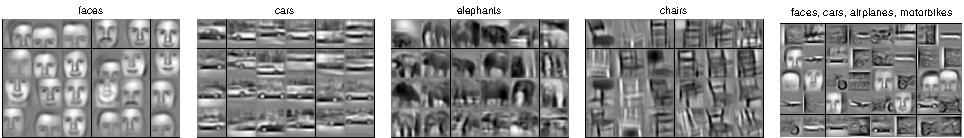
\includegraphics[width=\textwidth]{fig/rel/images/conv_layers.pdf}
    \caption{Filter response to learnt classes alongside CNN depth \autocite{lee2009convolutional}.}
    \label{fig:cnn_depth}
\end{figure}
\label{sec:oc_back}
Given a layer $\ell$ and a class of interest $c$, we consider saliency maps given by the general 
formula: \\

\begin{equation}
	S^c_\ell(\mathbf{u}) \defn h \left( \sum_k w^c_k A^k_\ell \right),
\label{eq:sal}
\end{equation}

where $w^c_k$ are weights defining a linear combination over channels and $h$ is an activation 
function, we present a visualization of this process in \autoref{fig:cam_schema}. It is through the 
calculation of these weights or weighting coefficients that a plethora of saliency methods have 
been proposed using CAM. Informally, this can be referred to as \emph{The Many Flavours of CAM}.
Moreover, given the flexibility in defining this coefficient, we outline milestone alternatives for 
this calculation.\\

\begin{figure}[t]
    \centering
        \begin{tikzpicture}[
            font={\footnotesize},
            trap/.style={trapezium, rotate=-90,trapezium angle=75},
        ]
            %% Nodes
            \node(input) at (-6, 0) {
\includegraphics[width=.1\textwidth]{fig/rel/images/cat_v2.jpg}};
            \node[above] at (input.north) {Input image $\vumod$};
            \node[draw, trap](cnn) at (-3, 0) {\rotatebox{90}{\parbox{1.0cm}{\centering{\Th{CNN}}}}};
            \node(fmaps) at (-0.5,0) {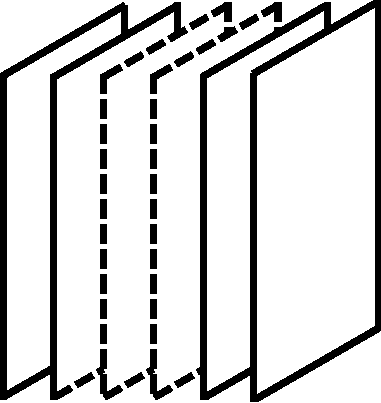
\includegraphics[width=.1\textwidth]{fig/rel/images/fmaps_side.pdf}};
            \node(fmk) at (-0.5, 1.3) {$A^k_\ell$};
            \node(classtag) at (3, 1.3) {\Th{Classifier}};
            \node(GAP) at (1.25,0.25) {$\gap$};
            \node(gapclass) at (3, 0) {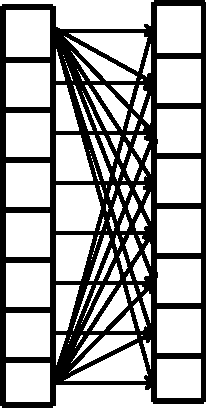
\includegraphics[width=.075\textwidth]{fig/rel/images/gapclass.pdf}};
            \node(logit) at (5, 0) {$\vy_c$};
            \node(wck) at (-0.5, -3) {
\includegraphics[width=0.02\textwidth, angle=90]{fig/rel/images/classifier.pdf}};
            \node(comb) at (-0.5, -3.5) {Weighting coefficient $w_k^c$};
            \node[draw, circle] (odot) at (-0.5, -1.8) {$\times$};
            \node(activ) at (-2.75, -1.5) {$h$};
            \node(salient) at (-3, -1.8) {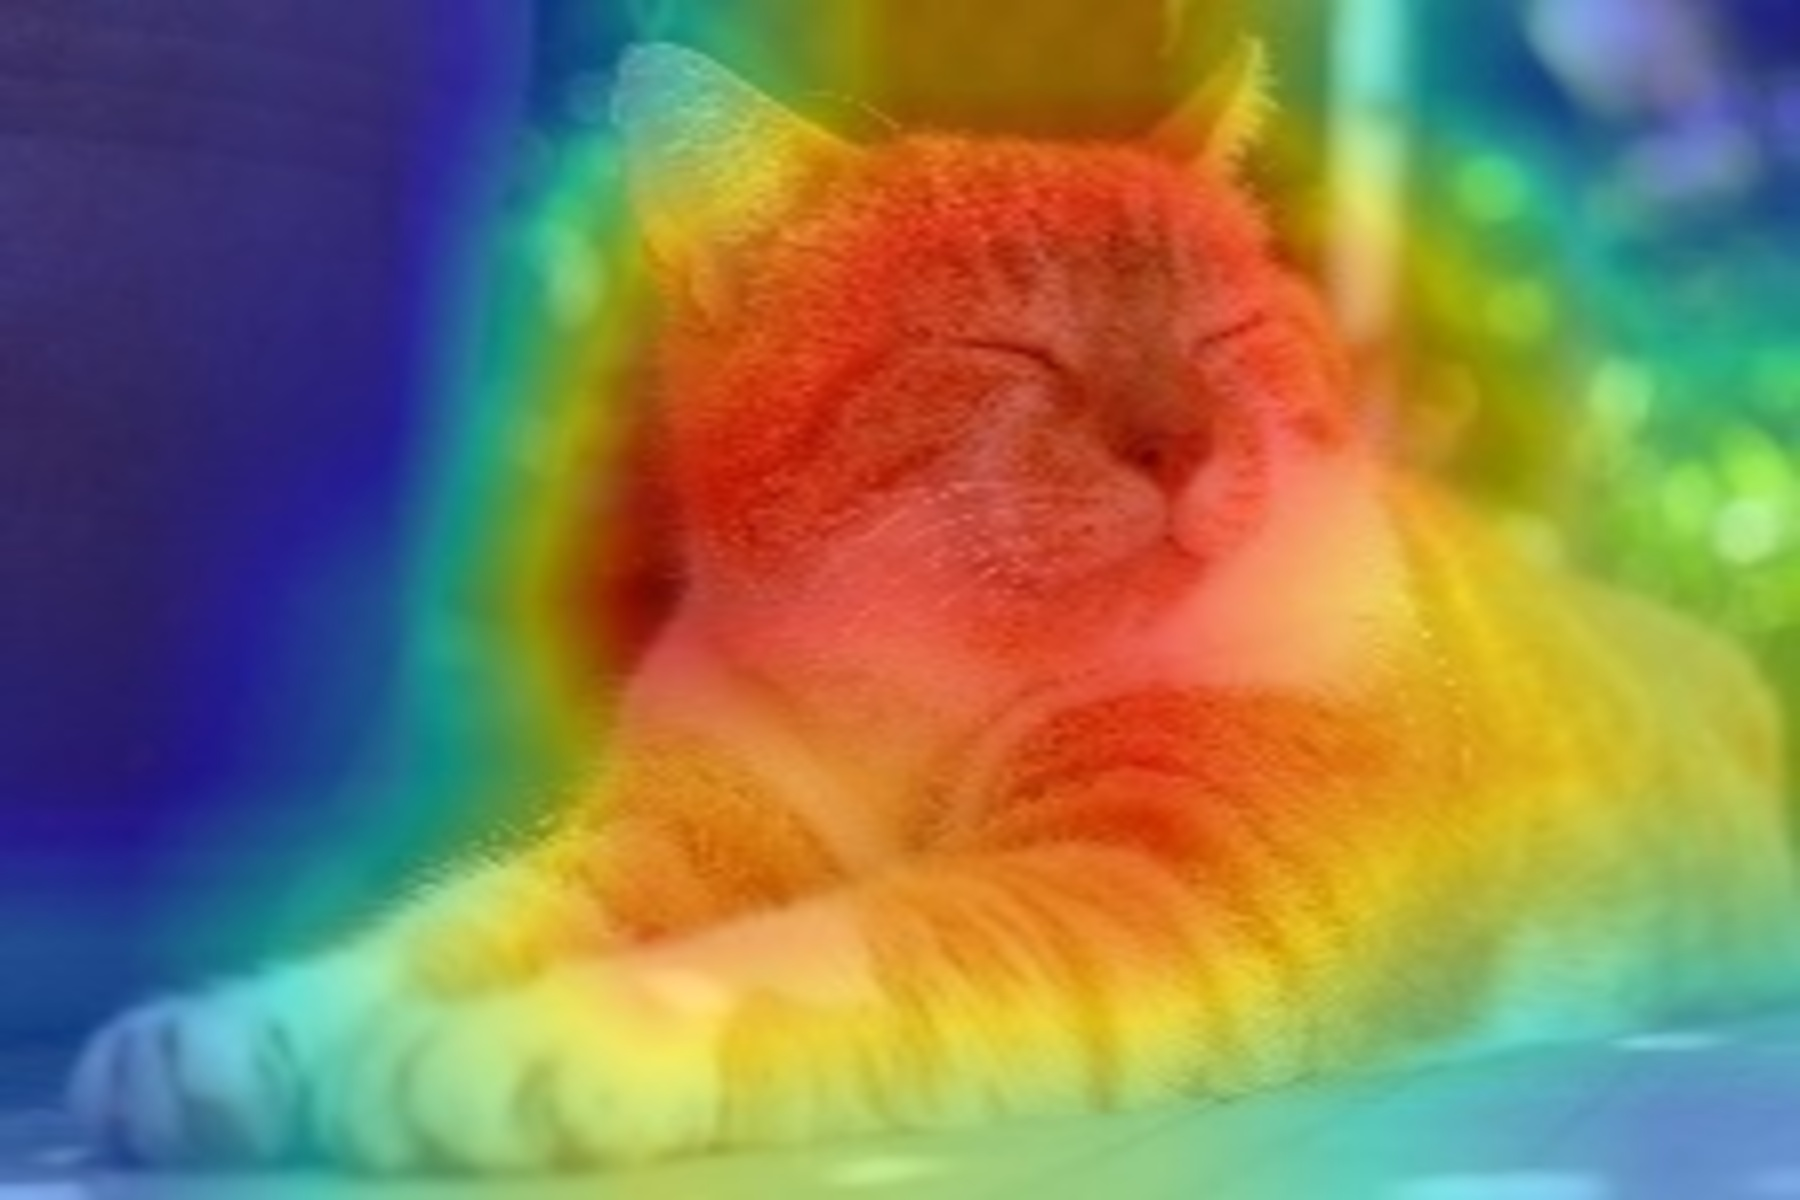
\includegraphics[width=.1\textwidth]{fig/rel/images/cat_cam.jpg}};
            \node[below] at (salient.south) {Saliency map $\mathbf{S_\ell}$};
            
            %% Edges

            \draw[->] (input.east) -- node {} (cnn);
            \draw[->] (cnn.north) -- node[above] {$\ell$} (fmaps.west);
            \draw[->] (fmaps.east) -- node {} (gapclass.west);
            \draw[->] (gapclass.east) -- node[above] {} (logit.west);
            \draw[->] (fmaps.south) -- node {} (odot.north);
            \draw[->] (wck.north) -- node {} (odot.south);
            \draw[->] (odot.west) -- node {} (salient);           

    \end{tikzpicture}
    \caption{\textbf{CAM} based methodologies overview.}
    \label{fig:cam_schema}
\end{figure}

\noindent \emph{CAM} \autocite{zhou2016learning} is the original proposal for this family of 
methods. This approach is defined uniquely for the last layer $L$ before the classifier and $h$ the 
identity mapping and $w^c_k$ is defined as the classifier weights that map the $k$-th channel in 
the feature map with class $c$. This first definition of class activation methods is not general, 
should a classifier be composed of a MLP; $w^c_k$ would have to account for the multiple 
interactions across the stages on the aforementioned layer, which ultimately is not 
straightforward. \\
 
\noindent\emph{Grad-CAM} \autocite{selvaraju2017grad} is proposed as a generalization of \emph{CAM}. 
Following the inconvenience of the calculation of the weighting coefficient on multi layered 
classifiers, this approach considers instead the flow of information on the network following the 
gradient generated by backpropagation following the logit of the class of interest. By doing so, 
the feature map to be used for an explanation can be selected from any
layer $\ell$ at different depths of the network. Moreover, the identity mapping on this approach is 
$h = \relu $ and the weighting coefficient is calculated in the following manner:
\begin{equation}
	w^c_k \defn \gap \left( \pder{y_c}{A^k_\ell} \right),
\label{eq:gcam_coeff}
\end{equation}
where $\gap$ is global average pooling.
The motivation for $\relu$ is that we are only interested in features that have a positive effect 
on the class of interest, \ie pixels whose intensity should be increased in order to increase $y_c$. 
Lastly, this approach also considers the computation of backpropagation using gradient refinements 
such as \emph{guided backpropagation} \autocite{guidedbackprop}, allowing for saliency maps to 
highlight more salient regions within the image.\\

\noindent \emph{Grad-CAM++} \autocite{chattopadhay2018grad} continues the trend of refining the 
generated saliency map via gradient modifications. In particular, the computation of the gradient 
follows partial derivatives as a way to address shortcomings on the original Grad-CAM. Specifically, 
Grad-CAM is not robust to multiple instances of the same clase within one image, and overall the 
localization of the attribution usually fails to be located over the entirety of the object of 
the class of interest. The computation of $w^c_k$ for Grad-CAM is defined in the following manner:
\begin{equation}
	w^c_k \defn \gap \left[\frac{\frac{\partial^2 y_c}{(\partial A^k)^2}}{2\frac{\partial^2 y_c}
	{(\partial A^k)^2}+\gap\left(A^k \frac{\partial^3 y_c}{(\partial A^k)^3}\right)}\right] \cdot 
	\relu \left(\pder{y^c}{A^k}\right)
	\label{eq:gcampp_coeff}
\end{equation}
Similar to Grad-CAM, Grad-CAM++ uses $h = \relu$, is not computational expensive, 
provides high quality saliency maps with better localization properties and is yet another 
generalization of prior approaches. Nevertheless, one crucial contribution proposed alongside this 
attribution method consists of an evaluation methodology for saliency maps, explained in detail in 
\autoref{rel:sub_evl}.\\

\noindent\emph{Score-CAM} \autocite{wang2020score} is also defined for any layer $\ell$ with 
$h = \relu$ and weights $w^c_k \defn \softmax(\mathbf{u}^c)_k$.  Softmax normalization considers 
positive channel contributions only and attends to few feature maps. Inspired by the idea of 
comparing the increase in confidence obtained by forwarding an image masked with the saliency map 
relating to class $c$, a vector $\mathbf{u}^c \in \real^{K_\ell}$ compares a known baseline image 
$\mathbf{u}_b$ with the input image $\mathbf{u}$, for all channels $k$:

\begin{equation}
	u^c_k \defn f(\mathbf{u} \odot n(\operatorname{up}( A^k_\ell )))_c - f(\mathbf{u}_b)_c,
\label{eq:s-cam}
\end{equation}

where $\odot$ is the Hadamard product. For this to work, the feature map $A^k_\ell$ is adapted 
to $\mathbf{u}$ first$:\operatorname{up}$ denotes upsampling to the spatial resolution of 
$\mathbf{u}$ and:

\begin{equation}
	n(A) \defn \frac{A - \min A}{\max A - \min A}
\label{eq:norm}
\end{equation}

is a normalization of matrix $A$ into $[0,1]$. While Score-CAM does not need gradients, it requires 
as many forward passes through the network as the number of channels in the chosen layer, which is 
computationally expensive. Score-CAM is better understood in a visual manner as in 
\autoref{fig:rel_sccam}\\

\begin{figure}[t]
    \centering
    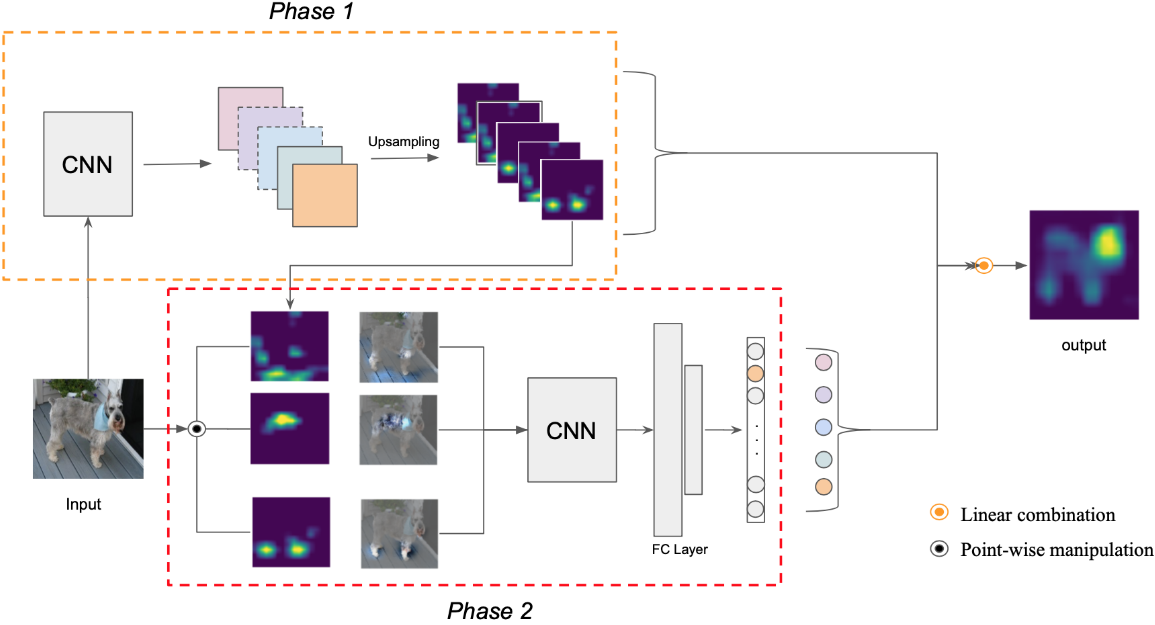
\includegraphics[width=\textwidth]{fig/rel/images/scorecam_schema.png}
    \caption{Score-CAM computation process \autocite{wang2020score}}
    \label{fig:rel_sccam}
\end{figure}
\noindent \emph{Axiom-CAM} \autocite{axiombased} Departing from the usage of the increase in 
confidence and gradient information, this approach incorporates logical principles to guide the 
calculation of the saliency map. In particular, two axioms are introduced \emph{sensitivity} and 
\emph{conservation}. On one hand \emph{sensitivity} considers that the importance of each feature 
map has to be equivalent to the score change caused by its removal. Conversely, \emph{conservation} 
points that changes in the saliency map come from a redistribution of the class score. In other 
words, sensitivity considers the loss of predictive power by the removal of high importance 
feature maps; \emph{conservation} instead ensures that class scores are mainly dominated by feature 
maps rather than external factors. By maintaining the activation function $h = \relu$, the 
formulation of the axiom-based weighting coefficient follows:

\begin{equation}
	w^c_k \defn \gap \left( \frac{A^k}{\gap(A^k)}\pder{y^c}{A^k}\right).
	\label{eq:ax_cam}
\end{equation}

\noindent \emph{Ablation-CAM} \autocite{ablationcam} continuing the trend of computing $w^c_k$ 
without making use of gradients, masking methods can be further incorporated in the production of 
saliency maps. More specifically, this approach determines the weight of individual feature maps 
via ablation perturbation. Going deeper, this approach evaluates the predictive power $y^c_k$ of an 
individual channel $k$ in feature map $A^k$ when all other activations are zeroed out. In one way, 
this could be een as similar to increase in confidence to produce the linear combination as in 
\emph{Score-CAM}. Nevertheless, in the current approach, modifications are done on feature space 
and the predictive power is compared with that of predictions using $A^k$ with all the feature maps 
unaltered. Retaining activation $h = \relu$, the formulation of this weighting coefficient follows:
\begin{equation}
	w^c_k \defn \frac{y^c-y^c_k}{y^c}
\end{equation}

\noindent \emph{Layer-CAM} \autocite{jiang2021layercam} although \gls{cam} can be extracted at any 
point of a model following the generalities described previously, they do not take into 
consideration the flow of information and relevant features along the depth of a model. 
Nevertheless, with backpropagation gradient can be probed alongside the whole depth of a model; as 
such, this approach computes a saliency map by averaging the upsampled attribution maps obtained at 
different depths from the model, generating a representation accounting for this information.

%--------------------------------------------------------------------------------------------------

%--------------------------------------------------------------------------------------------------
\subsection{Evaluating Interpretability}
\label{rel:sub_evl}
\paragraph Classification Metrics
\gls{ad} and \gls{ai} \autocite{chattopadhay2018grad} are 
well-established classification metrics. 
They measure the effect on the predicted class probabilities by masking the input image with the
 saliency map. Let $p^c_i$ and $o^c_i$ be the predicted probability for class $c$ given as input 
 the $i$-th test image $\vx_i$ and its masked version respectively. 
Masking refers to element-wise multiplication with the saliency map, which is at the same 
resolution as the original image with values in $[0,1]$. 
Let $N$ be the number of test images. Class $c$ is taken as the ground truth.

\emph{Average drop} (\gls{ad}) quantifies how much predictive power, measured as class probability, 
is lost when we only mask the image; lower is better:
\begin{equation}
	\AD(\%) \defn \frac{1}{N} \sum_{i=1}^N \frac{[p^c_i - o^c_i]_+}{p^c_i} \cdot 100.
\label{eq:ad}
\end{equation}

\emph{Average increase} (\gls{ai}), also known as \emph{increase in confidence}, measures the 
percentage of images where the masked image yiel ds a higher class probability than the original; 
higher is better:
\begin{equation}
	\AI(\%) \defn \frac{1}{N} \sum_i^N \mathbb{1}_{p^c_i < o^c_i} \cdot 100.
\label{eq:ai}
\end{equation}

$\AD$ and $\AI$ are not defined in a symmetric way. $\AD$ measures changes in class probability 
whereas $\AI$ measures a percentage of images. It is possible that the percentage is high while 
the actual increase is small. Hence, it is possible that an attribution method improves both. 
Indeed, \autocite{poppi2021revisiting} observes that a trivial method called Fake-CAM outperforms 
state-of-the-art methods, including Score-CAM, by a large margin. Fake-CAM simply defines a 
saliency map where the top-left pixel is set to zero and is uniform elsewhere. 
This questions the purpose of $\AD$ and $\AI$.

%--------------------------------------------------------------------------------------------------
\paragraph Localization metrics
\label{sec:loc-metrics}
Several works measure the localization ability of saliency maps, using metrics from the 
\emph{weakly-supervised object localization} (WSOL) task.

We are given the saliency map $S^c$ obtained from test image $\vx$ for ground truth class $c$. 
We denote by $S^c_{\vp}$ its value at pixel $\vp$. We binarize the saliency map by thresholding at 
its average value and we take the bounding box of the largest connected component of the resulting 
mask as the predicted bounding box $B_p$, represented as a set of pixels. We compare this box 
against the set of ground truth bounding boxes $\cB$, which typically contains 1 or 2 boxes of the 
same class $c$, or with their union $U = \cup \cB$, again represented as a set of pixels. We also 
compare the predicted class label $c_p$ with the ground truth label $c$. All metrics take values in 
$[0,1]$ and are expressed as percentages, except SM~\eq{sm}, which is unbounded.

\emph{Official Metric (OM)}
measures the maximum overlap of the predicted bounding box with any ground truth bounding box, 
requiring that the predicted class label is correct:
\begin{equation}
	\OM \defn 1 - \paren{\max_{B \in \cB} \iou(B, B_p)} \mathbbm{1}_{c_p = c},
\label{eq:om}
\end{equation}
where $\iou$ is intersection over union.
% is defined as $\iou(B, B_p) \defn \frac{B \cap B_p}{B \cup B_p}$.

\emph{Localization Error (LE)} is similar but ignores the predicted class label:
\begin{equation}
	\LE \defn 1 - \max_{B \in \cB} \iou(B, B_p).
\label{eq:le}
\end{equation}

\emph{Pixel-wise $F_1$ score (F1)} is defined as $F_1 = 2 \frac{P R}{P + R}$, where 
\emph{precision} $P$ is the fraction of mass of the saliency map that is within the ground truth 
union
\begin{equation}
	P \defn \frac{\sum_{\vp \in U} S^c_{\vp}}{\sum_{\vp} S^c_{\vp}}
\label{eq:prec}
\end{equation}

and \emph{recall} $R$ is the fraction of the ground truth union that is covered by the saliency map
\begin{equation}
	R \defn \frac{\sum_{\vp \in U} S^c_{\vp}}{\card{U}}.
	\label{eq:rec}
\end{equation}

\emph{Box Accuracy (BA)\autocite{choe2020evaluating}} Given threshold values $\eta$ and $\delta$, 
we find the bounding box $B^\eta_p$ of the largest connected component of the binary mask 
$\set{\vp: S_{\vp} > \eta}$ and require that it overlaps by 
$\delta$ with at least one ground truth box:
\begin{equation}
	\BA(\eta, \delta) \defn \max_{B \in \cB} \mathbbm{1}_{\iou(B^\eta_p, B) \ge \delta}.
\label{eq:ba}
\end{equation}
After averaging over the test images, we take the maximum of this measure over a set of values 
$\eta$ and then the average over a set of values $\delta$.\\
%--------------------------------------------------------------------------------------------------
\emph{Standard Pointing game (SP)\autocite{zhang2018top}} We find the pixel 
$\vp^* \defn \arg\max_{\vp} S^c_{\vp}$ having the maximum saliency value and 
require that it lands in any of the ground truth bounding boxes:
\begin{equation}
	\spg \defn \mathbbm{1}_{\vp^* \in U}.
\label{eq:spg}
\end{equation}\\

\emph{Energy Pointing game (EP)\autocite{wang2020score}} is equivalent to precision~\eq{prec}.\\

\emph{Saliency Metric (SM)\autocite{dabkowski2017real}} penalizes the size of the predicted bounding
 box $B_p$ relative to the image and the cross-entropy
 loss:
\begin{equation}
	\SM \defn \log \max\paren{ 0.05, \frac{\card{B_p}}{hw} } - \log p^c,
\label{eq:sm}
\end{equation}
where $h \times w$ is the input image resolution and $p^c$ is the precicted probability for ground 
truth class label $c$.

\subsection{Discussion}